\documentclass[10pt,unknownkeysallowed]{beamer}

\usetheme[progressbar=frametitle]{metropolis}
\usepackage{appendixnumberbeamer}
\usepackage{graphicx}
\usepackage{booktabs}
\usepackage[scale=2]{ccicons}

\usepackage{pgfplots}
\usepgfplotslibrary{dateplot}

\usepackage{xspace}
\newcommand{\themename}{\textbf{\textsc{metropolis}}\xspace}

\title{Spatial Autoregressive Models within GAMLSS}
\subtitle{Master Thesis}
% \date{\today}
\date{25/07/2019}
\author{Lucas de Miranda Oliveira}
\institute{UFPE}
% \titlegraphic{\hfill\includegraphics[height=1.5cm]{logo.pdf}}

\begin{document}

\maketitle

\begin{frame}{Outline}
  \setbeamertemplate{section in toc}[sections numbered]
  \tableofcontents[hideallsubsections]
\end{frame}

\section{Introduction}


\section{Elements}
\section{Simulations Study}
\begin{frame}{Medotolgy}
  \begin{figure}
\centering
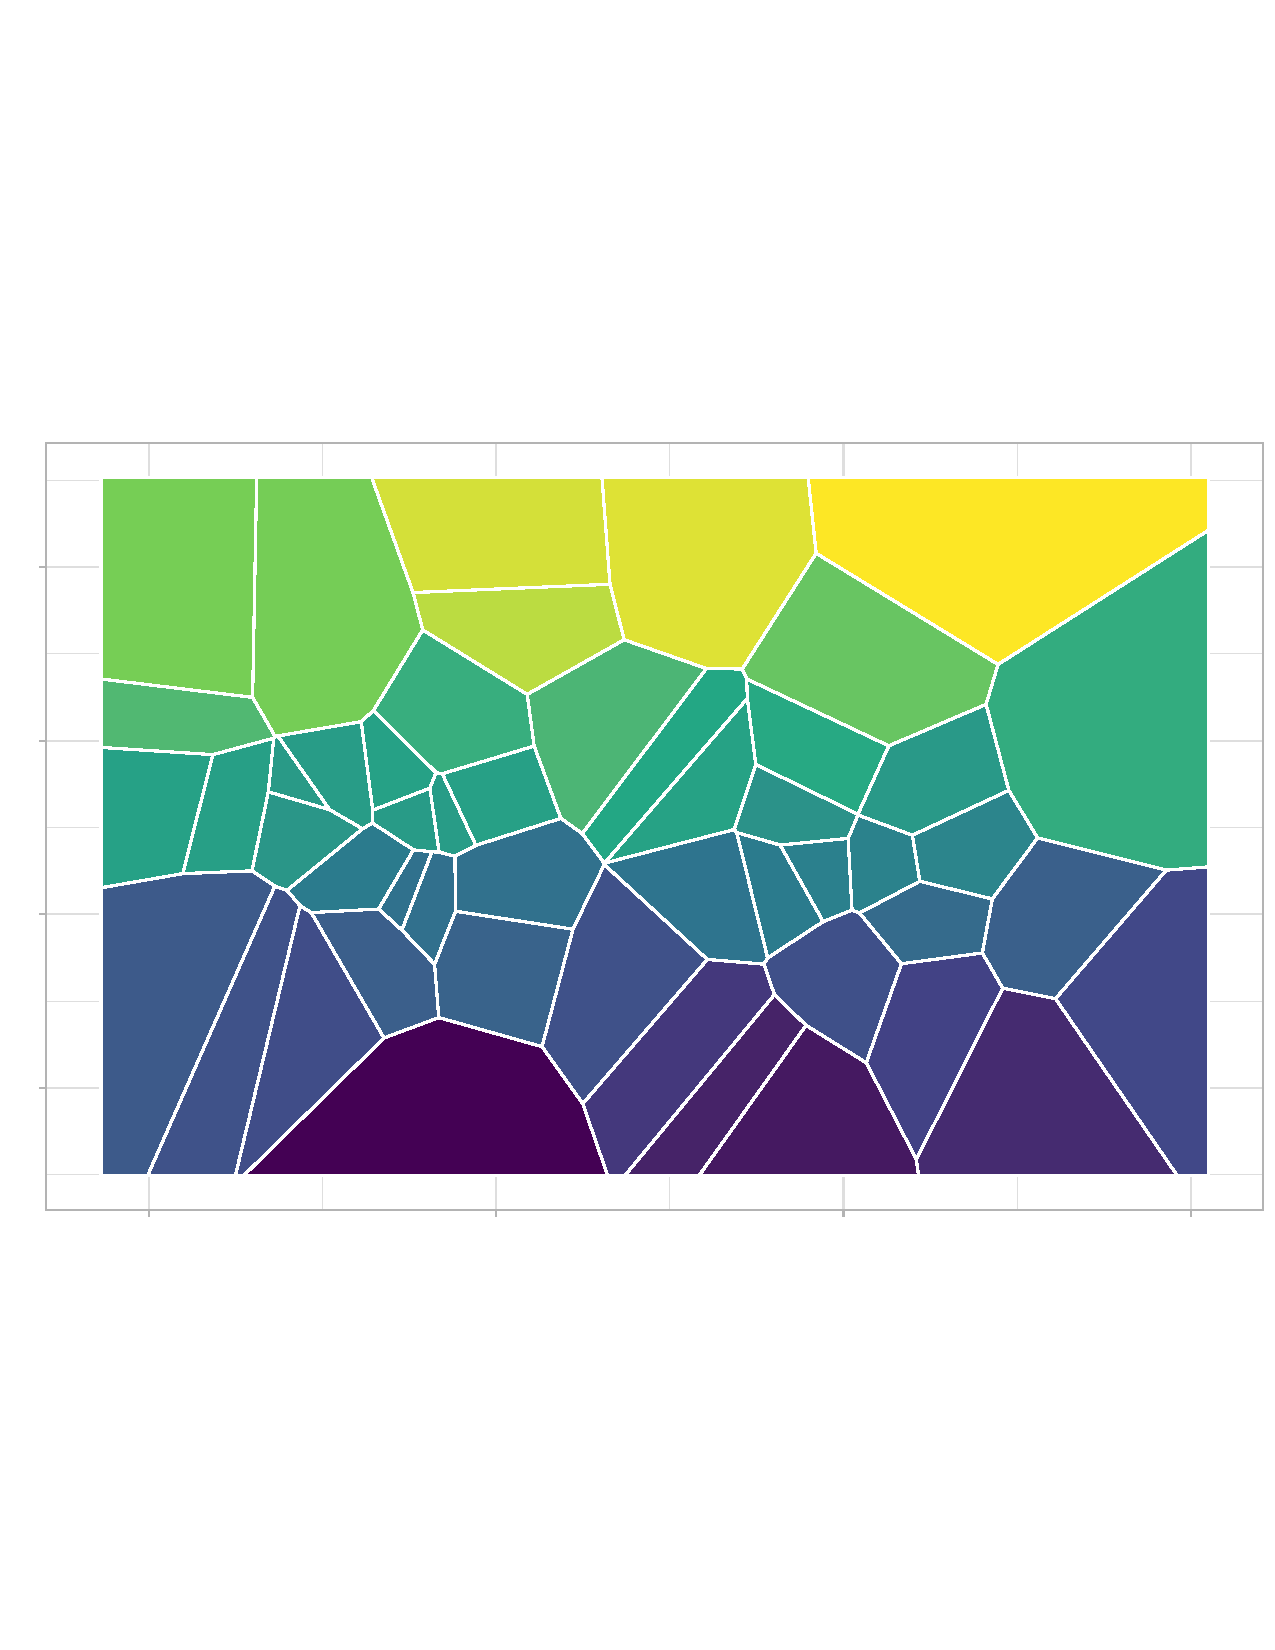
\includegraphics[width=0.7\linewidth]{VoroniDiagrams.pdf}
\caption{Voronoi}
\label{fig:Columbus_Sub}
\end{figure}
\end{frame}

\begin{frame}{Simulation based on Boston Housing \textit{data}}

Hedonic pricing data of Harrison and Rubinfeld (1978), in its corrected version (Gilley and Pace, 1996). In this article, the authors analyzed the demand for clean air through a hedonic price model for residences in Boston.

The variables are:
\begin{itemize}
    \item \texttt{PRICE}: logarithm of the median corrected value of household values in USD 1000's;
    \item \texttt{CRIM}: crime per capita in the town;
    \item \texttt{AGE}: the units occupied by the owners, proportionally, which were built before the year 1940;
    \item \texttt{NOX}: nitrogen oxides concentration;
    \item \texttt{RM}: average number of rooms per dwelling;
    \item  \texttt{ZN}: proportion of residential land zoned for lots over 25,000;
    \item  \texttt{INDUS}: proportion of non-retail business acres per town;
    \item \texttt{PTRATIO}: pupil-teacher ratio by town; 
    \item \texttt{RAD}: index of accessibility to radial highways;
    \item \texttt{TAX}: full-value property-tax rate per 10,000;
    \end{itemize}
    \end{frame}
    
    \begin{frame}{Simulation based on Boston Housing \textit{data}}
    \begin{itemize}
        \item \texttt{B}: $1000*(\textrm{Bk} - 0.63)^2$, where Bk is the proportion of blacks by town;
   \item \texttt{LSTAT}: lower status of the population;
   \item \texttt{DIS}:weighted mean of distances to five Boston employment centres 
    \end{itemize}
\end{frame}

\begin{frame}{ Design Experiment}
The simulation study based on real \textit{data} was performed as follows:
\begin{enumerate}
   \item Compute cholesky decomposition for a square matrix $\mat{\Sigma}$ of order $n$ such that $\mat{\Sigma}= \textbf{\textrm{L}}\textbf{\textrm{L}}^\top$ of the spatial structure present in the  \textit{data};
    \item  For each of the 1000 replicates of Monte Carlo a vector $\underline{\mat{\varepsilon}}$ of length $n$ is generated from uncorrelated normal random variables; and
    \item  Compute response variable $\underline{\mathbf{y}}$ with spatial dependency for each replicate by doing $\underline{\mat{y}}= \mat{\mu} + \textbf{\textrm{L}}\mat{\varepsilon}$, where $\mat{\mu} = \beta_0+ \beta_1\texttt{RM} + \beta_2\texttt{RAD}$, and $\textrm{Y}\sim \textrm{ Sinh-Arcsinh}(\mu,\sigma=1,\nu=0.5)$. The true values for $\underline{\beta}$ are
    $\underline{\beta}=(\beta_0,\beta_1,\beta2)=(1,0.5,0.5)$.
\end{enumerate}
\end{frame}

\begin{frame}{Results from simulation based on Boston Housing \textit{data}}
Figure \ref{fig:BostonBox} shows boxplots for estimates of parameters of regression.
\center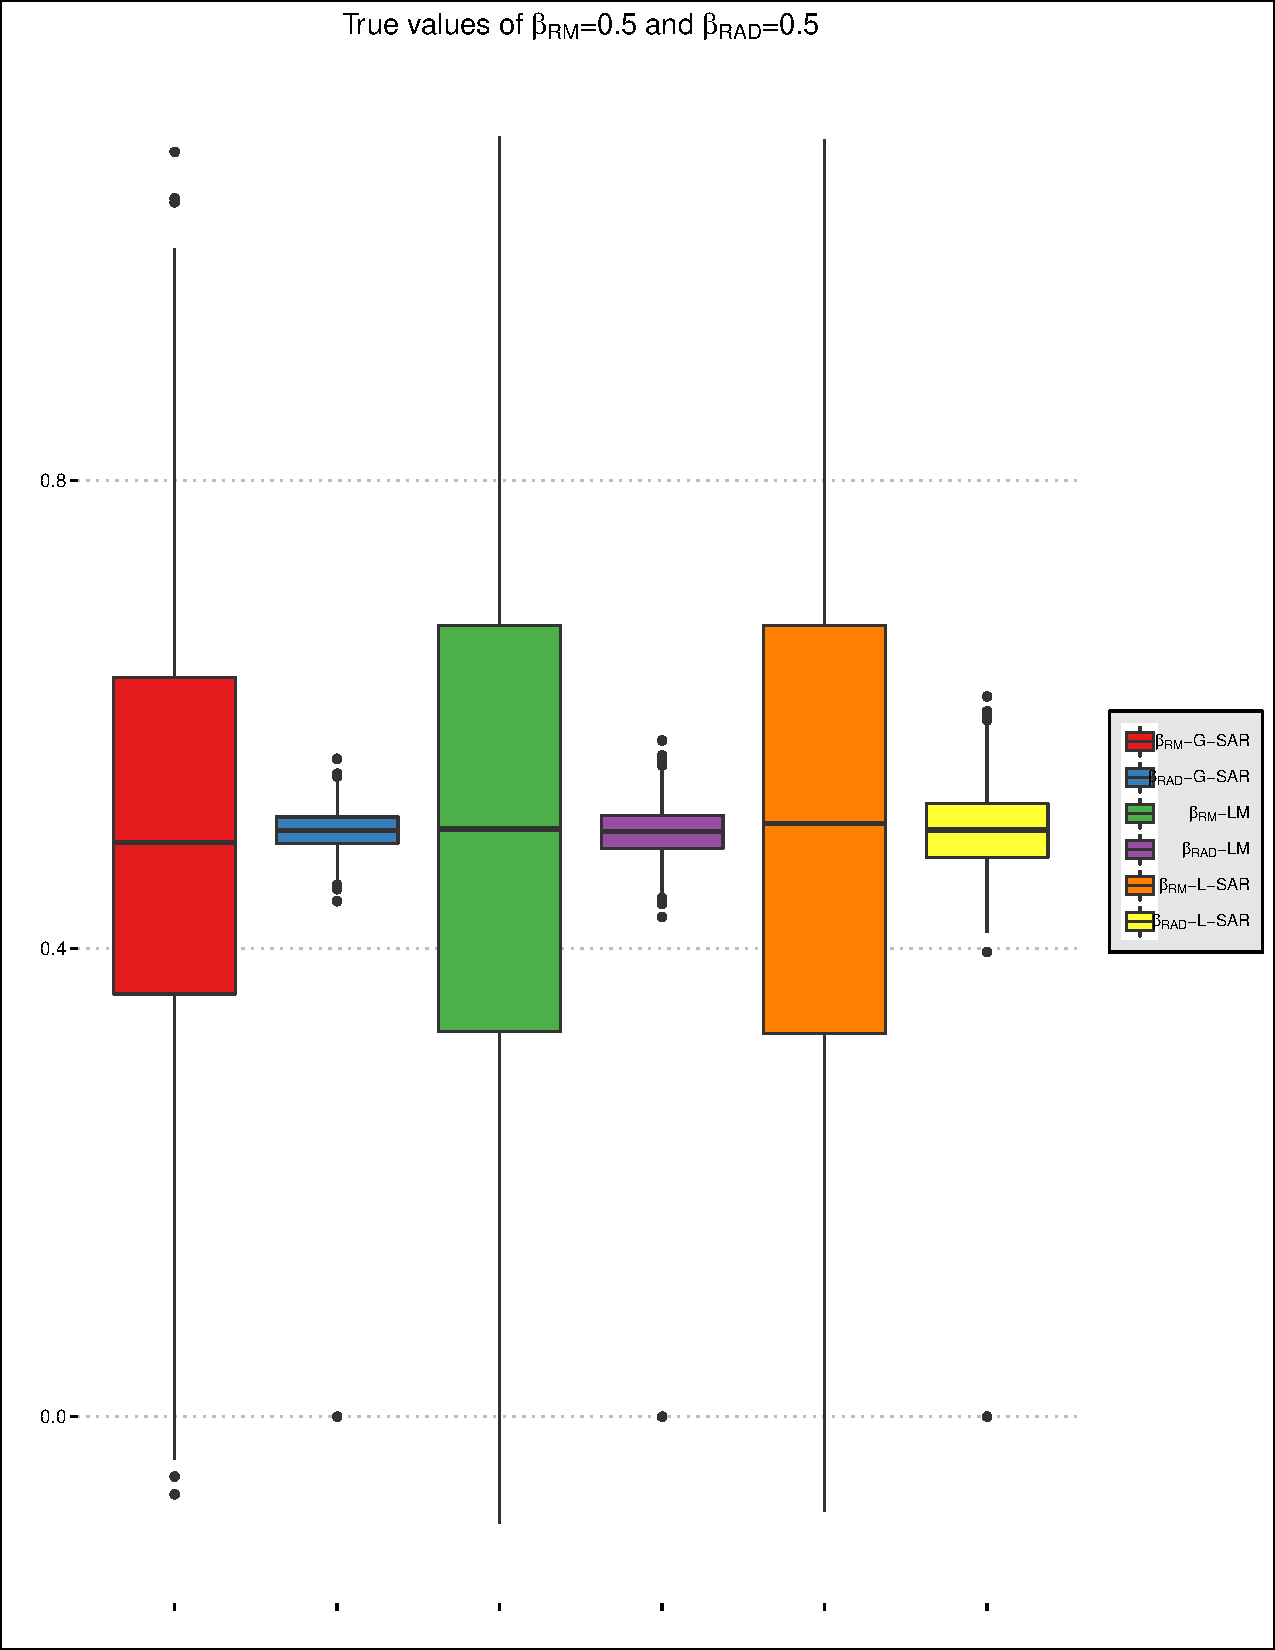
\includegraphics[width=4cm,height=5cm]{Betas_Boston_boxplot.pdf}\label{fig:BostonBox}
\end{frame}

\section{Applications}



\section{Conclusion}

{\setbeamercolor{palette primary}{fg=black, bg=yellow}
\begin{frame}[standout]
  Questions?
\end{frame}
}


\begin{frame}[allowframebreaks]{References}

  \bibliography{demo}
  \bibliographystyle{abbrv}

\end{frame}

\end{document}